% Канонический TikZ-рисунок варианта 06. Править только здесь.
\long\def\figStereoV06{%
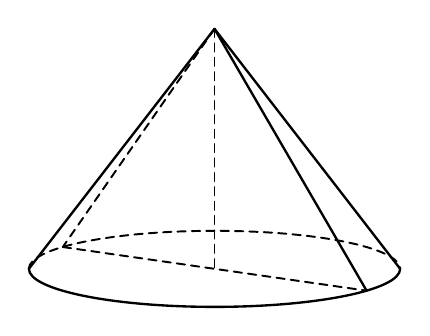
\begin{tikzpicture}[
    scale=1.15,
    line cap=round,
    line join=round,
    visible/.style={
        line width=0.85pt
    },
    hidden/.style={
        line width=0.7pt,
        dashed,
        dash pattern=on 3pt off 2.2pt
    }
]

% -------------------------------------------------
% Параметры изображения
% -------------------------------------------------

\def\R{2.05}    % горизонтальный радиус эллипса
\def\r{0.42}    % вертикальный радиус эллипса
\def\H{2.65}    % изображаемая высота конуса

% -------------------------------------------------
% Основные точки
% -------------------------------------------------

\coordinate (S) at (0,\H);   % вершина конуса
\coordinate (O) at (0,0);    % центр основания

% Крайние точки основания
\coordinate (L) at (-\R,0);
\coordinate (R) at ( \R,0);

% Концы диаметра осевого сечения
\coordinate (P) at
    ({(\R+1.3)*cos(120)},{\r*sin(145)});

\coordinate (Q) at
    ({\R*cos(-35)},{\r*sin(-35)});

% -------------------------------------------------
% Задняя половина основания
% -------------------------------------------------

\draw[hidden]
    (L)
    arc[
        start angle=180,
        end angle=0,
        x radius=\R,
        y radius=\r
    ];

% -------------------------------------------------
% Скрытая образующая осевого сечения
% -------------------------------------------------

\draw[hidden] (S)--(P);

% Диаметр основания в плоскости осевого сечения
\draw[hidden] (P)--(Q);

% Ось конуса
\draw[hidden] (S)--(O);

% -------------------------------------------------
% Внешние образующие конуса
% -------------------------------------------------

\draw[visible] (S)--(L);
\draw[visible] (S)--(R);

% Видимая образующая осевого сечения
\draw[visible] (S)--(Q);

% -------------------------------------------------
% Передняя половина основания
% -------------------------------------------------

\draw[visible]
    (R)
    arc[
        start angle=0,
        end angle=-180,
        x radius=\R,
        y radius=\r
    ];

\end{tikzpicture}
}
